\documentclass[tikz,border=8pt]{standalone}
\usetikzlibrary{arrows.meta}

\begin{document}
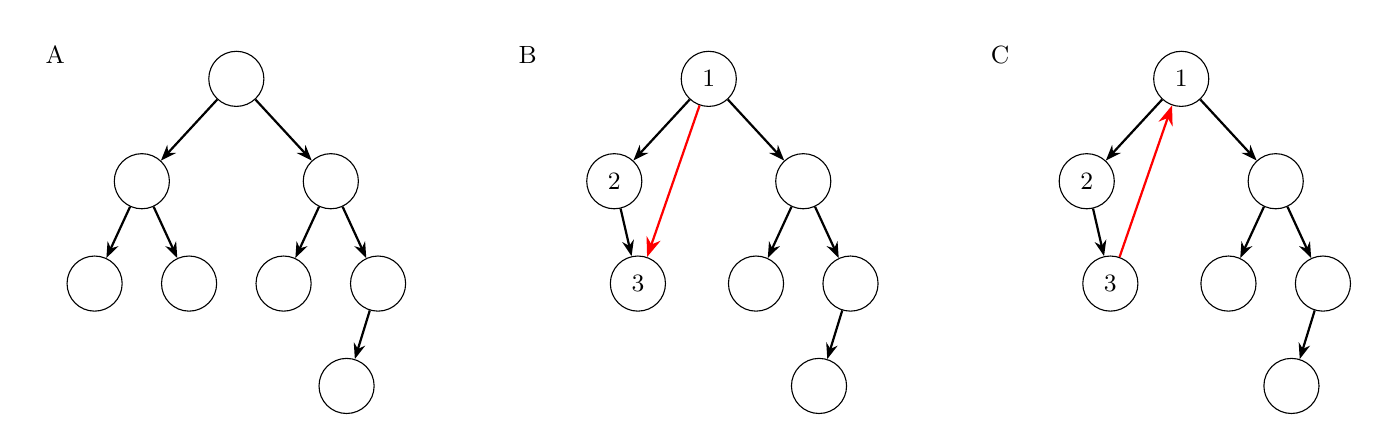
\begin{tikzpicture}[
  every node/.style={circle, draw, minimum size=7mm, inner sep=0pt, font=\small},
  edge/.style={-{Stealth[length=2mm]}, thick},
  redarrow/.style={-{Stealth[length=2.5mm]}, red, thick}
]

% ---------- Tree A ----------
\begin{scope}
  \node[draw=none] at (-2.3,0.3) {A};
  \node (Aroot) at (0,0)        {};
  \node (AL)    at (-1.2,-1.3)  {};
  \node (AR)    at (1.2,-1.3)   {};
  \node (ALL)   at (-1.8,-2.6)  {};
  \node (ALR)   at (-0.6,-2.6)  {};
  \node (ARL)   at (0.6,-2.6)   {};
  \node (ARR)   at (1.8,-2.6)   {};
  \node (ARRC)  at (1.4,-3.9)   {};

  \draw[edge] (Aroot) -- (AL);
  \draw[edge] (Aroot) -- (AR);
  \draw[edge] (AL) -- (ALL);
  \draw[edge] (AL) -- (ALR);
  \draw[edge] (AR) -- (ARL);
  \draw[edge] (AR) -- (ARR);
  \draw[edge] (ARR) -- (ARRC);
\end{scope}

% ---------- Tree B (arrow 1 -> 3) ----------
\begin{scope}[xshift=6cm]
  \node[draw=none] at (-2.3,0.3) {B};
  \node (Broot) at (0,0)        {1};
  \node (BL)    at (-1.2,-1.3)  {2};
  \node (BR)    at (1.2,-1.3)   {};
  \node (B3)    at (-0.9,-2.6)  {3};
  \node (BRL)   at (0.6,-2.6)   {};
  \node (BRR)   at (1.8,-2.6)   {};
  \node (BRRC)  at (1.4,-3.9)   {};

  \draw[edge] (Broot) -- (BL);
  \draw[edge] (Broot) -- (BR);
  \draw[edge] (BL) -- (B3);
  \draw[edge] (BR) -- (BRL);
  \draw[edge] (BR) -- (BRR);
  \draw[edge] (BRR) -- (BRRC);

  \draw[redarrow] (Broot) -- (B3);
\end{scope}

% ---------- Tree C (arrow 3 -> 1) ----------
\begin{scope}[xshift=12cm]
  \node[draw=none] at (-2.3,0.3) {C};
  \node (Croot) at (0,0)        {1};
  \node (CL)    at (-1.2,-1.3)  {2};
  \node (CR)    at (1.2,-1.3)   {};
  \node (C3)    at (-0.9,-2.6)  {3};
  \node (CRL)   at (0.6,-2.6)   {};
  \node (CRR)   at (1.8,-2.6)   {};
  \node (CRRC)  at (1.4,-3.9)   {};

  \draw[edge] (Croot) -- (CL);
  \draw[edge] (Croot) -- (CR);
  \draw[edge] (CL) -- (C3);
  \draw[edge] (CR) -- (CRL);
  \draw[edge] (CR) -- (CRR);
  \draw[edge] (CRR) -- (CRRC);

  \draw[redarrow] (C3) -- (Croot);
\end{scope}

\end{tikzpicture}
\end{document}
